\chapter{Introducción y marco teórico}

\section{Contexto del problema computacional}

Los árboles binarios de búsqueda (BST, \textit{Binary Search Tree}) constituyen una de las estructuras más didácticas y, al mismo tiempo, más traicioneras de la computación moderna. Su invariante es elegante: para todo nodo $u$, las claves del subárbol izquierdo son menores que $\mathrm{key}(u)$ y las del subárbol derecho son mayores. Esa propiedad habilita búsquedas que, en el caso ideal, descienden por la altura del árbol en tiempo $\bigO(\log n)$.

El problema aparece cuando la secuencia de inserciones no es aleatoria. Insertar claves ordenadas $1, 2, 3, \ldots, n$ produce un árbol degenerado: una lista enlazada disfrazada de árbol. La altura pasa a ser $n-1$ y cada búsqueda cuesta $\bigO(n)$. Durante décadas, la respuesta dominante fue introducir \textbf{factores de balance} en cada nodo (AVL, Red-Black) y corregir desviaciones mediante \textbf{rotaciones locales}.

En 1993, Galperin y Rivest propusieron un enfoque radicalmente distinto en su artículo \textit{Scapegoat Trees}. En lugar de mantener balance incremental con rotaciones, permiten que el árbol se desbalancee temporalmente y, cuando la profundidad excede un umbral teórico, identifican un nodo \textbf{scapegoat} (chivo expiatorio) cuyo subárbol se \textbf{reconstruye completamente} en orden balanceado. No hay rotaciones. No hay campos de balance por nodo. El precio se paga en reconstrucciones que pueden tocar $\bigO(n)$ nodos en una operación aislada, pero cuyo costo \textbf{amortizado} permanece logarítmico bajo distribuciones razonables de operaciones.

Este informe documenta la implementación completa de esa estructura en Go, su integración con SQL Server como capa de persistencia, la exposición de una API REST para mutaciones y consultas, y una interfaz Vue.js que visualiza el comportamiento del algoritmo ---incluyendo la selección del scapegoat y la reconstrucción del subárbol--- en tiempo casi real.

\section{El paper de Galperin y Rivest (1993)}

\subsection{Problema fundacional}

En la década de 1990, las estructuras balanceadas dominantes (AVL, Red-Black, B-Trees) habían madurado, pero compartían una característica: \textbf{cada nodo almacena información adicional} para decidir cuándo y cómo rotar. Galperin y Rivest se preguntaron si era posible obtener altura $\bigO(\log n)$ amortizada \textbf{sin} almacenar metadatos de balance en los nodos y \textbf{sin} rotaciones.

\subsection{Definición formal}

Sea $T$ un \Scapegoat{} parametrizado por $\alpha \in (0.5, 1)$. El árbol mantiene dos contadores globales:

\begin{table}[H]
  \centering
  \caption{Contadores del algoritmo Scapegoat}
  \begin{tabular}{@{}cl@{}}
    \toprule
    \textbf{Símbolo} & \textbf{Definición} \\
    \midrule
    $n$ & Número actual de nodos \\
    $q$ & Máximo valor de $n$ alcanzado desde la última reconstrucción global \\
    \bottomrule
  \end{tabular}
\end{table}

La \textbf{profundidad máxima permitida} tras una inserción, dado el valor actual de $q$, es:
\begin{equation}
  d_{\max}(q) = \left\lfloor \log_{1/\alpha}(q) \right\rfloor
  \label{eq:dmax}
\end{equation}

Cuando la profundidad del nodo recién insertado supera $d_{\max}(q)$, el algoritmo asciende por el \textbf{camino de inserción} desde la hoja hacia la raíz buscando el nodo padre $p$ tal que:
\begin{equation}
  \mathrm{size}(\mathrm{hijo}) > \alpha \cdot \mathrm{size}(p)
  \label{eq:scapegoat-cond}
\end{equation}

donde $\mathrm{size}(u)$ denota el número de nodos en el subárbol raíz en $u$. Ese padre $p$ es el \textbf{scapegoat}. Su subárbol completo se aplana mediante un recorrido in-order, se almacena en un arreglo temporal y se reconstruye como un BST \textbf{perfectamente balanceado} seleccionando el elemento medio como raíz del subárbol.

Para la eliminación, el paper adopta una política más drástica: \textbf{no} se buscan scapegoats. Si tras eliminar un nodo se cumple:
\begin{equation}
  n < \alpha \cdot q
  \label{eq:global-rebuild}
\end{equation}
entonces se reconstruye \textbf{todo el árbol} y se asigna $q \leftarrow n$.

\subsection{Diagrama del algoritmo de inserción}

\begin{figure}[H]
  \centering
  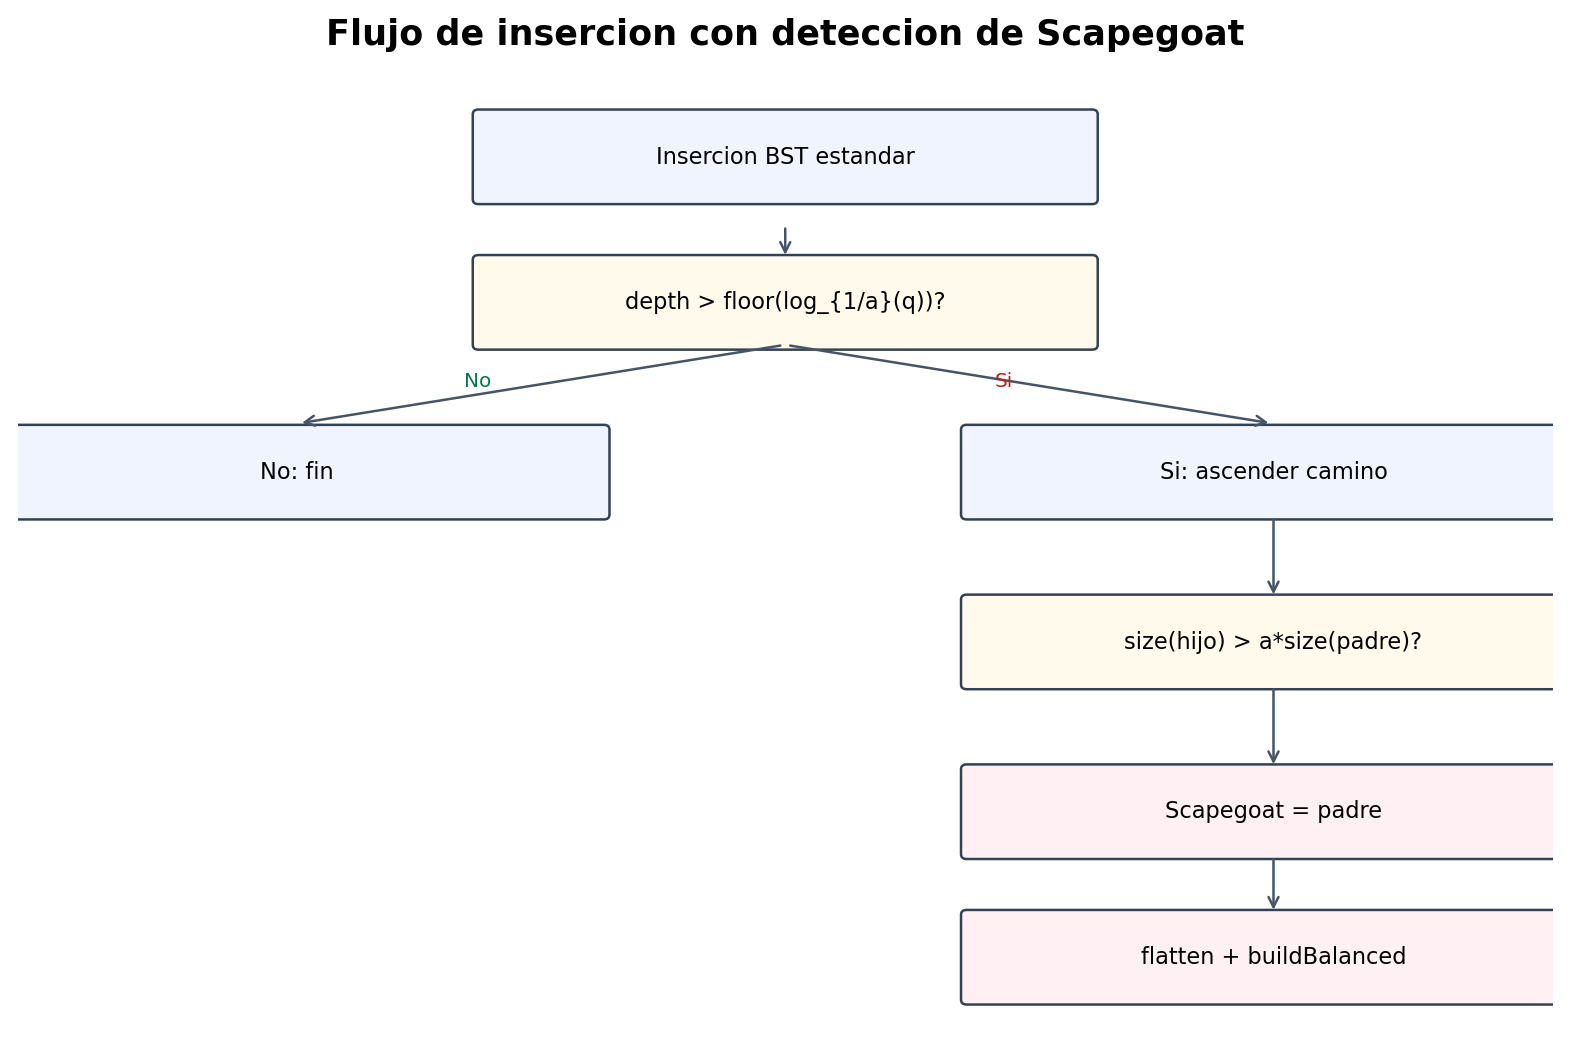
\includegraphics[width=0.92\textwidth]{diagrams/02-flujo-insercion.png}
  \caption{Flujo de inserción con detección de Scapegoat}
  \label{fig:flujo-insercion}
\end{figure}

\begin{figure}[H]
  \centering
  \begin{tikzpicture}[
    node distance=0.55cm and 1.1cm,
    startstop/.style={rectangle, rounded corners, draw=esanblue, fill=blue!8, minimum width=2.8cm, align=center, font=\small},
    decision/.style={diamond, draw=orange!70!black, fill=orange!10, aspect=2, inner sep=1pt, align=center, font=\footnotesize},
    arrow/.style={-{Stealth[length=2mm]}, thick}
  ]
    \node[startstop] (a) {Insertar clave $k$};
    \node[decision, below=of a] (b) {¿Árbol vacío?};
    \node[startstop, below left=0.9cm and 1.4cm of b] (c) {Crear raíz\\$n{=}1$, $q{=}1$};
    \node[startstop, below right=0.9cm and 1.4cm of b] (d) {Descender BST};
    \node[decision, below=of d] (e) {¿$\mathrm{depth} > d_{\max}(q)$?};
    \node[startstop, below left=of e] (f) {Fin};
    \node[startstop, below right=of e] (g) {Buscar scapegoat\\rebuild subárbol};
    \draw[arrow] (a) -- (b);
    \draw[arrow] (b) -- node[left, font=\scriptsize]{Sí} (c);
    \draw[arrow] (b) -- node[right, font=\scriptsize]{No} (d);
    \draw[arrow] (d) -- (e);
    \draw[arrow] (e) -- node[left, font=\scriptsize]{No} (f);
    \draw[arrow] (e) -- node[right, font=\scriptsize]{Sí} (g);
  \end{tikzpicture}
  \caption{Representación esquemática TikZ del algoritmo de inserción}
  \label{fig:tikz-insercion}
\end{figure}

\subsection{Invariantes y teoremas}

\begin{invariante}[Altura débil]
Mientras $n \geq \alpha \cdot q$ o tras una reconstrucción global, la altura del árbol está acotada por $d_{\max}(q) + \bigO(1)$.
\end{invariante}

\begin{teorema}[Galperin \& Rivest]
Una secuencia de $m$ operaciones de inserción y eliminación sobre un \Scapegoat{} con parámetro $\alpha$ tiene costo total $\bigO(m \log n)$, siendo el costo amortizado por operación $\bigO(\log n)$.
\end{teorema}

\section{Justificación frente a alternativas}

\begin{table}[H]
  \centering
  \caption{Comparación con AVL y Red-Black}
  \begin{tabular}{@{}lcc@{}}
    \toprule
    \textbf{Criterio} & \textbf{AVL / Red-Black} & \textbf{Scapegoat Tree} \\
    \midrule
    Metadato por nodo & Factor de balance o color & Ninguno \\
    Mecanismo de balance & Rotaciones locales & Reconstrucción de subárbol \\
    Peor operación individual & $\bigO(\log n)$ & $\bigO(n)$ \\
    Amortizado & $\bigO(\log n)$ & $\bigO(\log n)$ \\
    Complejidad de código & Alta & Media \\
    \bottomrule
  \end{tabular}
\end{table}

Frente al \texttt{map} nativo de Go, que ofrece $\bigO(1)$ amortizado pero no mantiene orden, el \Scapegoat{} expone \texttt{InOrder()} en $\bigO(n)$ y preserva la topología BST para fines pedagógicos. Frente a Skip Lists, nuestra elección es \textbf{determinista}, lo que simplifica pruebas y simulación visual.
